% Copyright (C) 2012 Shi.Zhan <g.shizhan.g@gmail.com>
%
% Permission is hereby granted, free of charge, to any person obtaining a copy of this software and associated documentation files (the "Software"), to deal in the Software without restriction, including without limitation the rights to use, copy, modify, merge, publish, distribute, sublicense, and/or sell copies of the Software, and to permit persons to whom the Software is furnished to do so, subject to the following conditions:
%
% The above copyright notice and this permission notice shall be included in all copies or substantial portions of the Software.
%
% THE SOFTWARE IS PROVIDED "AS IS", WITHOUT WARRANTY OF ANY KIND, EXPRESS OR IMPLIED, INCLUDING BUT NOT LIMITED TO THE WARRANTIES OF MERCHANTABILITY, FITNESS FOR A PARTICULAR PURPOSE AND NONINFRINGEMENT. IN NO EVENT SHALL THE AUTHORS OR COPYRIGHT HOLDERS BE LIABLE FOR ANY CLAIM, DAMAGES OR OTHER LIABILITY, WHETHER IN AN ACTION OF CONTRACT, TORT OR OTHERWISE, ARISING FROM, OUT OF OR IN CONNECTION WITH THE SOFTWARE OR THE USE OR OTHER DEALINGS IN THE SOFTWARE.
%
% 课程:人机交互技术及应用
% 班级:传播学1001班
% 课时:40学时,2012年秋季1~10周,每周一、三
% 地点:东九楼D212
% 主页:http://code.google.com/p/hci-course/
% 教师:施展 
% 单位:华中科技大学 武汉光电国家实验室
%
\documentclass{beamer}
\usepackage{fontspec,xunicode,xltxtra,beamerthemesplit}
%\usetheme{Hannover} % White background
\usetheme{Berkeley} % Blue background
\setsansfont[Mapping=tex-text, ItalicFont={Courier Italic}]{Microsoft YaHei}

% 中文环境自动换行
\XeTeXlinebreaklocale "zh"
\XeTeXlinebreakskip = 0pt plus 1pt

% 中文环境修正导航栏
\makeatletter
\def\beamer@linkspace#1{
	\begin{pgfpicture}{0pt}{-1.5pt}{#1}{5.5pt}
		\pgfsetfillopacity{0}
		\pgftext[x=0pt,y=-1.5pt]{.}
		\pgftext[x=#1,y=5.5pt]{.}
	\end{pgfpicture}
}
\makeatother

% diagrams
\usepackage{tikz}

\tikzset{
	every overlay node/.style={
		anchor=north west,
	},
}
% Usage:
% \tikzoverlay at (-1cm,-5cm) {content};
% or
% \tikzoverlay[text width=5cm] at (-1cm,-5cm) {content};
\def\tikzoverlay{%
	\tikz[baseline,overlay]\node[every overlay node]
}%

\title{人机交互技术}
\author{施展}
\institute{华中科技大学~武汉光电国家实验室}
\date{\today}
\titlegraphic{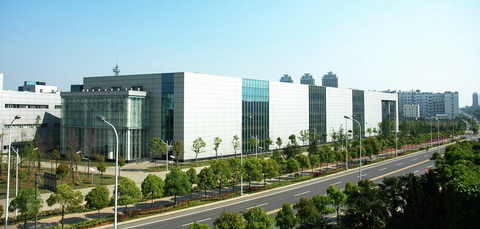
\includegraphics[width=2cm]{images/wnlo.jpg}}

\begin{document}

\begin{frame}
	\titlepage
\end{frame}

\begin{frame}
	\frametitle{内容提要}
	\tableofcontents
\end{frame}

\section{第三讲}
\begin{frame}
	\frametitle{第三讲 交互设备}
	\begin{itemize}
%		\item 了解文本输入设备,图像输入设备,指点输入设备,掌握三维图形输入设备
		\item 了解文本输入设备,图像输入设备,触摸屏输入设备,体感输入设备
%		\item 了解显示器,声音的输出,数字纸等输出设备
		\item 了解显示器,声音的输出,电子墨水等输出设备
%		\item 了解虚拟现实交互设备
	\end{itemize}
\end{frame}

\subsection{输入设备}
\begin{frame}
	\frametitle{输入设备}
	\begin{center}
	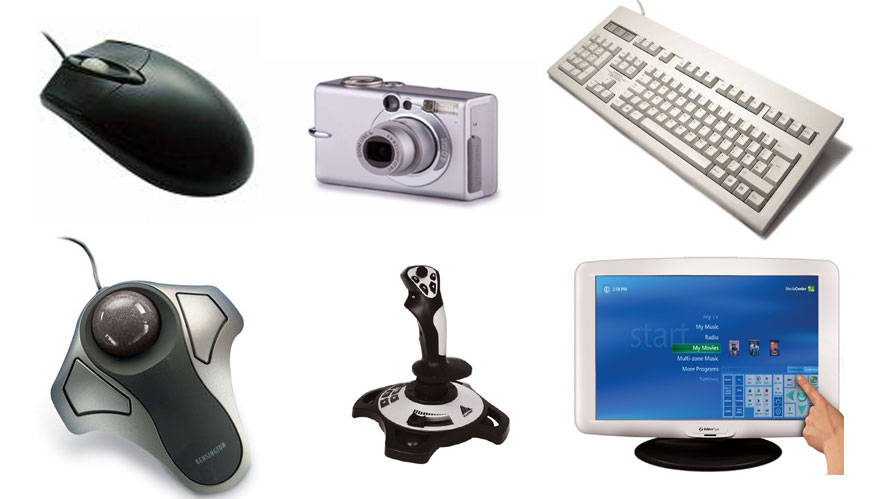
\includegraphics[width=\textwidth]{images/input-devices.jpg}
	\end{center}
\end{frame}

\subsubsection{文本输入设备}
\begin{frame}
	\frametitle{文本输入设备}
	\begin{itemize}
		\item 文本输入是人与计算机交互的一个重要组成部分,同时也是一项繁重的工作。
		\begin{itemize}
			\item 键盘为主
			\item 手写、识别(字符/条码、图像、语音)为辅
		\end{itemize}
	\end{itemize}
\end{frame}

\begin{frame}
	\frametitle{键盘 Keyboard}
	\tikzoverlay at (0cm,-3cm) {{\tiny 文本输入最主要手段,应用环境影响布局,布局影响速度、准确性、舒适度。}};
	\tikzoverlay at (1.5cm, 4cm) {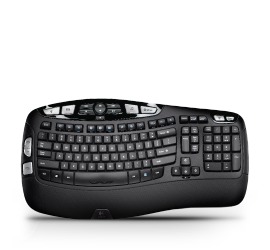
\includegraphics[width=5cm]{images/keyboard.png}};
	\tikzoverlay at (0cm, 0cm) {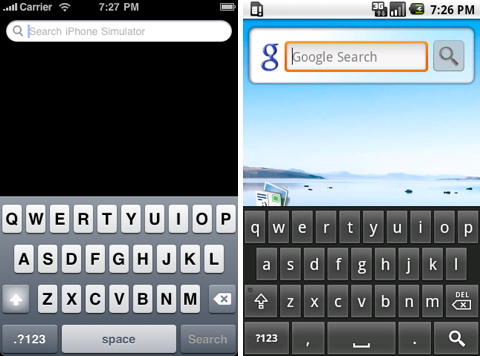
\includegraphics[width=3cm]{images/mobile_keyboards.png}};
	\tikzoverlay at (6cm, 0cm) {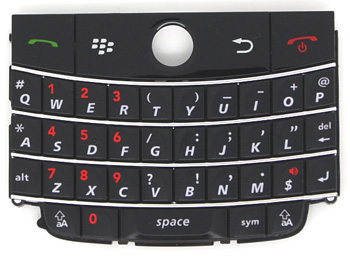
\includegraphics[width=3cm]{images/blackberry-bold-9000-keyboard.jpg}};
\end{frame}

\begin{frame}
	\frametitle{键盘分类}

\end{frame}

\begin{frame}
	\frametitle{键盘布局}

\end{frame}

\begin{frame}
	\frametitle{人机工程学键盘}

\end{frame}

\begin{frame}
	\frametitle{多功能集成键盘}

\end{frame}

\begin{frame}
	\frametitle{手写设备}

\end{frame}

\begin{frame}
	\frametitle{手写笔}

\end{frame}

\begin{frame}
	\frametitle{手写板}

\end{frame}

\begin{frame}
	\frametitle{光学字符识别 Optical Character Recognition}

\end{frame}

\begin{frame}
	\frametitle{手写汉字识别 Handwriting Recognition}

\end{frame}

\subsubsection{指点输入设备}
\begin{frame}
	\frametitle{指点输入设备}
	\begin{itemize}
		\item 指点设备常用于完成一些定位和选择物体的交互任务。
		\item 物体可能处于一维、二维、三维或更高维的空间中。
		\item 选择与定位的方式可以是直接选择,或通过操作屏幕上的光标来完成。
	\end{itemize}
\end{frame}

\begin{frame}
	\frametitle{鼠标 Mouse}

\end{frame}

\begin{frame}
	\frametitle{鼠标的分类}

\end{frame}

\begin{frame}
	\frametitle{鼠标与计算机的接口}

\end{frame}

\begin{frame}
	\frametitle{鼠标的结构}

\end{frame}

\begin{frame}
	\frametitle{新型鼠标}

\end{frame}

\begin{frame}
	\frametitle{触摸板 Touchpad}

\end{frame}

\begin{frame}
	\frametitle{控制杆 Joy Stick}

\end{frame}

\begin{frame}
	\frametitle{触摸屏 Touch Screen}

\end{frame}

\begin{frame}
	\frametitle{触摸屏的组成与分类}

\end{frame}

\begin{frame}
	\frametitle{多点触摸}

\end{frame}

\subsubsection{图像输入设备}
\begin{frame}
	\frametitle{图像输入设备}

\end{frame}

\begin{frame}
	\frametitle{扫描仪}

\end{frame}

\begin{frame}
	\frametitle{数码摄像头}

\end{frame}

\subsection{输出设备}
\begin{frame}
	\frametitle{输出设备}

\end{frame}

\subsubsection{显示器}
\begin{frame}
	\frametitle{显示器}

\end{frame}

\subsubsection{打印机}
\begin{frame}
	\frametitle{打印机}

\end{frame}

\subsubsection{电子墨}
\begin{frame}
	\frametitle{电子墨}

\end{frame}

\subsubsection{语音交互设备}
\begin{frame}
	\frametitle{语音交互设备}

\end{frame}

\section{小结}
\begin{frame}
	\frametitle{小结}
	\begin{itemize}
		\item 输入设备:
		\begin{itemize}
			\item 文本输入设备
			\item 图像输入设备
			\item 指点输入设备\dots
		\end{itemize}
		\item 输出设备:
		\begin{itemize}
			\item 显示器 
			\item 打印机
			\item 声音的输出\dots
		\end{itemize}
	\end{itemize}
\end{frame}
 
\begin{frame}
	\frametitle{参考文献}
	\bibliographystyle{plain}
	\bibliography{hci}
\end{frame}

\end{document}